\section[Теория]{Онтология предметной области}
\subsection{Структура рабочего места}

\begin{frame}{Структурная схема системы и объекта контроля}
    \begin{minipage}[t]{0.57\linewidth}
        \textbf{Пример рабочего места}
        \center{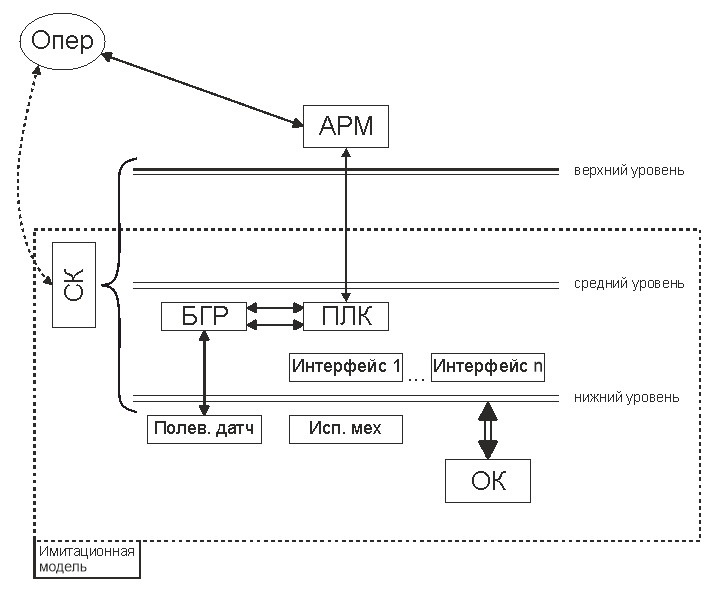
\includegraphics[width=1\linewidth,keepaspectratio]{scheme_3levels}}
    \end{minipage}
    \hfill
    \begin{minipage}[t]{0.4\linewidth}
        \begin{itemize}
            \item[АРМ] автоматизированное рабочее место
            \item[БГР] блок гальванической развязки
            \item[ОК]  объект контроля
            \item[ПЛК] программируемый логический контроллер
            \item[СК]  система контроля            
        \end{itemize}
    \end{minipage}\pause
    \vspace{5mm}
    \centering{\fbox{\parbox{.8\textwidth}{АНПА предназначен для поиска скоплений \textit{планктона},
                \textit{рыбных косяков} или \textit{китов} путем анализа испущенной специализированной зондирующей посылки.}}}
\end{frame}
\note{
    Рассказ об устройстве СК и связях с ОК
}

\begin{frame}{Четырехуровневая модель метаданных}
    \begin{minipage}[t]{0.4\linewidth}
    \centering
    \begin{tabular}{cc}
    \toprule
    \textbf{Уровень} & \textbf{Название} \\ \midrule
        3 & Мета-метакласс \\\hline
        2 & Метакласс      \\\hline
        1 & Класс          \\\hline
        0 & Объект         \\\hline
    \bottomrule
    \end{tabular}
\end{minipage}
\hfill\vrule
\begin{minipage}[t]{0.55\linewidth}
    \centering
    \begin{itemize}
        \item RDF описывает структуру данных
        \item Метакласс
        \item Класс
        \item \texttt{C1} (Внешнее питание, \texttt{true}, 8001)
    \end{itemize}
\end{minipage}
    % \cite{journal:vestnik_spbgu:ivakin,book:gost:56272,w3c:rdf:lassila}
\end{frame}

\section[Анализ]{Декомпозиция АНПА}
\begin{frame}{Материальная составляющая модели АНПА}
    \center{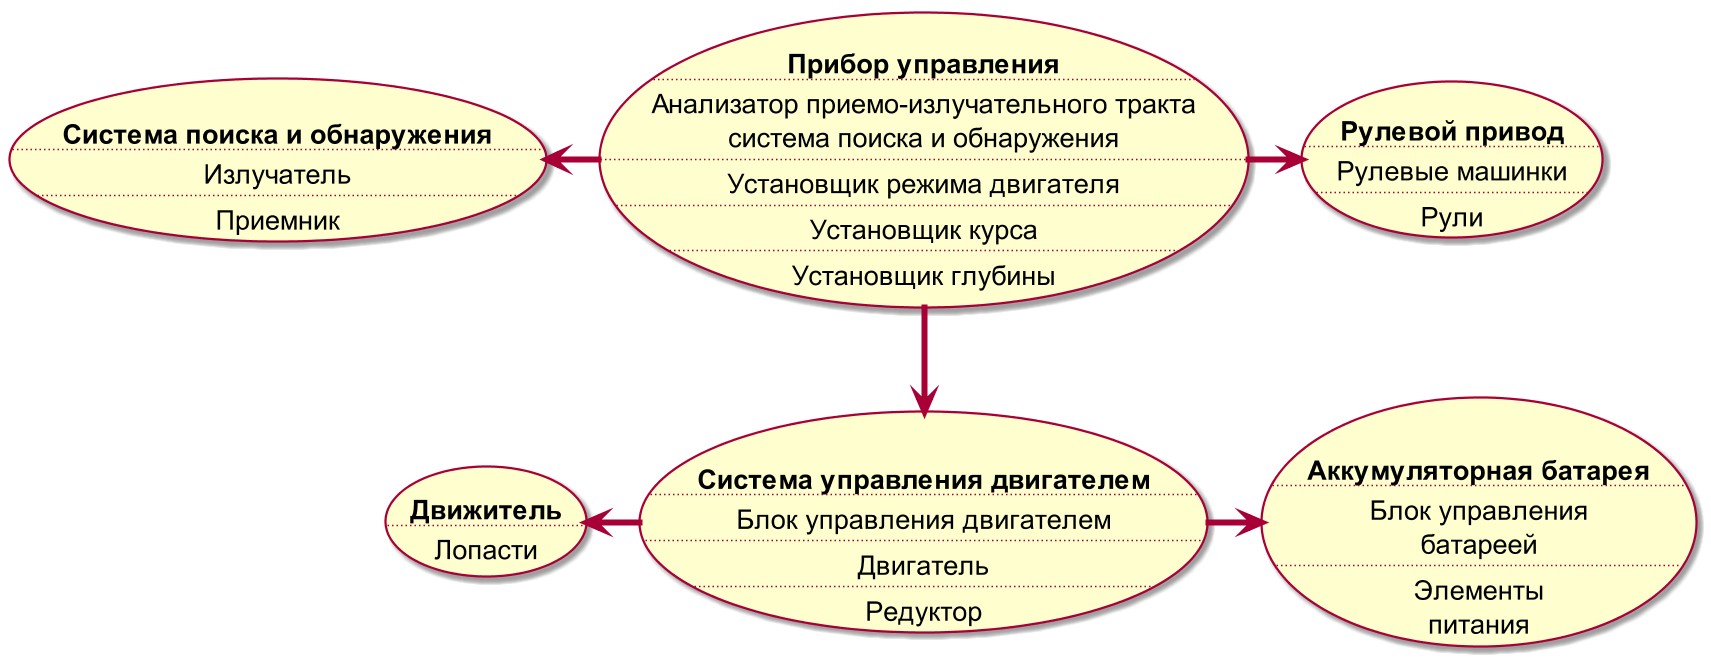
\includegraphics[width=1\linewidth,keepaspectratio]{model_anpa}}
\end{frame}
\note{
}


\begin{frame}{Объект -- Функция -- Действие}{\small Графоаналитический метод для выявления общесистемных сущностей.}
\small{\cite{journal:vestnik_igeu:elizarova}}
\tiny\begin{tabular}{cp{.2\textwidth}||c|p{.15\textwidth}||cp{.15\textwidth}}
    \toprule
    \multicolumn{2}{|c||}{\textbf{Объект}} & \multicolumn{2}{c||}{\textbf{Функции}} & \multicolumn{2}{c|}{\textbf{Действия}} \\ \midrule
    %
    \multicolumn{1}{|l|}{\multirow{2}{*}{СПО}} & Излучатель                                  & \multirow{5}{*}{Движение}          & Вперед                           & \multicolumn{1}{l|}{\multirow{3}{*}{ПУ}}  & \multicolumn{1}{l|}{Пеленгация целей}     \\ \cline{2-2} \cline{4-4} \cline{6-6}
    \multicolumn{1}{|l|}{}                     & Приемник                                    &                                    & Вправо                           & \multicolumn{1}{l|}{}                     & \multicolumn{1}{l|}{Коррекция курса}      \\ \cline{1-2} \cline{4-4} \cline{6-6}
    \multicolumn{1}{|l|}{\multirow{4}{*}{ПУ}}  & Анализатор приемо-излучательного тракта СПО &                                    & Влево                            & \multicolumn{1}{l|}{}                     & \multicolumn{1}{l|}{Коррекция глубины}    \\ \cline{2-2} \cline{4-4} \cline{5-6}
    \multicolumn{1}{|l|}{}                     & Установщик режима двигателя                 &                                    & Вверх                            & \multicolumn{1}{l|}{\multirow{2}{*}{АКБ}} & \multicolumn{1}{l|}{Хранение}             \\ \cline{2-2} \cline{4-4} \cline{6-6}
    \multicolumn{1}{|l|}{}                     & Установщик курса                            &                                    & Вниз                             & \multicolumn{1}{l|}{}                     & \multicolumn{1}{l|}{Доставка}             \\ \cline{2-6}
    \multicolumn{1}{|l|}{}                     & Установщик глубины                          & \multirow{5}{*}{Питание}           & СПО                              & \multicolumn{1}{l|}{Д}                    & \multicolumn{1}{l|}{Толкает водную среду} \\ \cline{1-2} \cline{4-6}
    \multicolumn{1}{|l|}{\multirow{3}{*}{СУД}} & БУД                                         &                                    & ПУ                               &                                           &                                           \\ \cline{2-2} \cline{4-4}
    \multicolumn{1}{|l|}{}                     & Двигатель                                   &                                    & СУД                              &                                           &                                           \\ \cline{2-2} \cline{4-4}
    \multicolumn{1}{|l|}{}                     & Редуктор                                    &                                    & РП                               &                                           &                                           \\ \cline{1-2} \cline{4-4}
    \multicolumn{1}{|l|}{\multirow{2}{*}{РП}}  & РМ                                          &                                    & Д                                &                                           &                                           \\ \cline{2-4}
    \multicolumn{1}{|l|}{}                     & Рули                                        & \multirow{2}{*}{Обнаружение}       & Излучение зондирующей посылки    &                                           &                                           \\ \cline{1-2} \cline{4-4}
    \multicolumn{1}{|l|}{Д}                    & Лопасти                                     &                                    & Прием отраженого сигнала         &                                           &                                           \\ \cline{1-4}
    \multicolumn{1}{|l|}{\multirow{2}{*}{АКБ}} & БУБ                                         & \multirow{4}{*}{Принятие решений}  & Изменить скорость движения       &                                           &                                           \\ \cline{2-2} \cline{4-4}
    \multicolumn{1}{|l|}{}                     & Модули питания                              &                                    & Изменить курс                    &                                           &                                           \\ \cline{1-2} \cline{4-4}
                                               &                                             &                                    & Изменить глубину хода            &                                           &                                           \\ \cline{4-4}
                                               &                                             &                                    & Изменить тип зондирующей посылки &                                           &                                           \\ \cline{3-4}
\end{tabular}
    \begin{minipage}[t]{0.4\linewidth}
        \centering
            Матрицы связности: 
            \begin{itemize}
                \item[$A$] взаимосвязь \textbf{Объект -- Функция} \pause
                \item[$B$] взаимосвязь \textbf{Функция -- Действие} \pause
                \item[$C_1 = A \times B$] взаимосвязь \textbf{Объект -- Действие} \pause
            \end{itemize}
    \end{minipage}
    \hfill
    \begin{minipage}[t]{0.55\linewidth}
        \vspace{1pt} $C_2 = \begin{pmatrix} \sum_{j=1}^l c_{1\,1j} \\ \ldots \\ \sum_{j=1}^l c_{1\,mj} \\ \end{pmatrix}\!; \quad C_3 = \left. \frac{C_2}{l} \right|_{l \equiv 6}$
    \end{minipage}
\end{frame}

\begin{frame}
    \tiny
    \begin{equation*}
        \begin{split}
        A = &\begin{pmatrix}
            0 & 0 & 0 & 0 & 0 & 1 & 0 & 0 & 0 & 0 & 1 & 0 & 0 & 0 & 0 & 0 \\
            0 & 0 & 0 & 0 & 0 & 1 & 0 & 0 & 0 & 0 & 0 & 1 & 0 & 0 & 0 & 0 \\
            0 & 0 & 0 & 0 & 0 & 1 & 1 & 0 & 0 & 0 & 0 & 1 & 0 & 0 & 0 & 1 \\
            0 & 0 & 0 & 0 & 0 & 0 & 0 & 1 & 0 & 1 & 0 & 0 & 0 & 0 & 0 & 0 \\
            0 & 1 & 1 & 0 & 0 & 0 & 0 & 0 & 0 & 0 & 1 & 0 & 0 & 1 & 0 & 1 \\
            0 & 0 & 0 & 1 & 1 & 0 & 0 & 0 & 0 & 0 & 0 & 0 & 0 & 0 & 1 & 0 \\
            0 & 0 & 0 & 0 & 0 & 1 & 0 & 0 & 0 & 0 & 0 & 0 & 1 & 0 & 0 & 0 \\
            0 & 0 & 0 & 0 & 0 & 1 & 0 & 0 & 0 & 0 & 0 & 0 & 1 & 0 & 0 & 0 \\
            0 & 0 & 0 & 0 & 0 & 0 & 0 & 0 & 0 & 1 & 0 & 0 & 0 & 0 & 0 & 0 \\
            1 & 1 & 1 & 1 & 1 & 0 & 0 & 0 & 0 & 0 & 0 & 0 & 0 & 1 & 1 & 0 \\
            1 & 1 & 1 & 1 & 1 & 0 & 0 & 0 & 0 & 0 & 0 & 0 & 0 & 1 & 1 & 0 \\
            0 & 0 & 0 & 0 & 0 & 0 & 0 & 0 & 0 & 0 & 0 & 0 & 0 & 1 & 1 & 0 \\
            0 & 0 & 0 & 0 & 0 & 1 & 1 & 1 & 1 & 1 & 1 & 0 & 0 & 0 & 0 & 0 \\
            0 & 0 & 0 & 0 & 0 & 0 & 0 & 0 & 0 & 0 & 1 & 1 & 0 & 0 & 0 & 0 \\
        \end{pmatrix},{}\\
    %
        B = &\begin{pmatrix}
            0 & 0 & 0 & 0 & 0 & 0 & 0 & 0 & 0 & 0 & 1 & 1 & 0 & 0 & 0 & 1 \\
            0 & 1 & 1 & 0 & 0 & 0 & 0 & 0 & 0 & 0 & 0 & 1 & 1 & 1 & 0 & 0 \\
            0 & 0 & 0 & 1 & 1 & 0 & 0 & 0 & 0 & 0 & 0 & 0 & 1 & 0 & 1 & 0 \\
            0 & 0 & 0 & 0 & 0 & 1 & 1 & 1 & 1 & 1 & 0 & 0 & 0 & 0 & 0 & 0 \\
            0 & 0 & 0 & 0 & 0 & 1 & 1 & 1 & 1 & 1 & 1 & 0 & 0 & 0 & 0 & 1 \\
            1 & 0 & 0 & 0 & 0 & 0 & 0 & 0 & 0 & 0 & 0 & 0 & 1 & 1 & 1 & 0 \\
        \end{pmatrix}^T\,,{}\\
    %
        C_1 = A \times B = &\begin{pmatrix}
            1 & 1 & 2 & 0 & 2 & 0 & 0 & 0 & 0 & 0 & 0 & 0 & 1 & 2 \\
            0 & 1 & 1 & 0 & 3 & 0 & 1 & 1 & 0 & 3 & 3 & 1 & 0 & 1 \\
            0 & 0 & 0 & 0 & 0 & 3 & 1 & 1 & 0 & 3 & 3 & 1 & 0 & 0 \\
            1 & 1 & 2 & 2 & 0 & 0 & 1 & 1 & 1 & 0 & 0 & 0 & 5 & 0 \\
            2 & 1 & 3 & 2 & 2 & 0 & 1 & 1 & 1 & 0 & 0 & 0 & 6 & 1 \\
            0 & 0 & 0 & 0 & 1 & 1 & 1 & 1 & 0 & 3 & 3 & 2 & 0 & 0 \\
        \end{pmatrix}^T\,,{}\\
    %
        C_3 = &\left. \frac{C_2}{l} \right|_{l \equiv 6} = 
            \left( 0.67\;\; 0.67\;\; \textbf{1.33}\;\; 0.67\;\; \textbf{1.33}\;\; 0.67\;\; 0.83\;\; 0.83\;\; 
            0.33\;\; \textbf{1.50}\;\;\textbf{1.50}\;\; 0.67\;\; \textbf{2.00}\;\; 0.67 \right)^T\,.
    \end{split}
    \end{equation*} 

    Пороговое значение $K_{min} = \overline{C_3} = 0.98$
    \begin{itemize}
        \item[2.0]   блок управления батареей;
        \item[1.5]   рулевые машинки, рулевой привод;
        \item [1.33] анализатор приемо-излучательного тракта СПО и установщик курса.
    \end{itemize}
\end{frame}

\begin{frame}{Имитируемые сигналы}
    \textbf{Общесистемные сущности}:
    \begin{itemize}
        \item<1->[2.0]   блок управления батареей;
        \item<1->[1.5]   рулевые машинки, рулевой привод;
        \item<1->[1.33] анализатор приемо-излучательного тракта СПО и установщик курса.
    \end{itemize}
    %
    \begin{enumerate}
        \item<2-> Внешние
        \begin{itemize}
            \item<2->[Глубина] $\{t_1, t_2, \ldots, t_n\} \rightarrow \{h_1, h_2, \ldots, h_n\}$;
            \item<3->[Эхо-сигнал] $s_j \Rightarrow \{r_{j1}, r_{j2}, \ldots, r_{jn}\} \equiv \{r_j\} \cup \{e_j\}$, причем $\{r_j\} \cap \{e_j\} = \emptyset$,
                где $\{e_j\}$ -- множество аварийных ответов.
        \end{itemize}\hrule{}\vspace{5pt}
        \item<4-> Внутренние
        \begin{itemize}
            \item<4->[Напряжения] $U_i = \{U_1, U_2, \ldots, U_j\};\quad U_i \in [U_i^{min}, U_i^{max}]$
            \item<4->[Токи] $I_\Sigma = \sum_k^N I_k + \hat I;\quad I_k \in [I_k^{min}, I_k^{max}];\quad \hat I \in [\hat I^{min}, \hat I^{max}]$
            \item<5->[СУД] $\langle f; Q \rangle$ вращения вала \textit{двигателя} в виде ШИМ сигнала
            \item<6->[Руление] $\langle s_j, \{r_j\} \rangle \Rightarrow \omega_i = \omega_i(s_j, \{r_j\}), i\in [1..N]$
        \end{itemize}    
    \end{enumerate}
\end{frame}
\note{}


\begin{frame}{Онтология модели АНПА}
        \begin{center}
            % \begin{tikzpicture}[scale=.6,transform shape]
            %     \begin{scope}
            %         \only<1>{
            %             \tikzstyle{VertexStyle}=[ellipse,draw=black, line width=1,font=\bfseries]
            %             \tikzstyle{LabelStyle}=[font=\bfseries,fill=gray!20,sloped,rectangle, rounded corners, draw]
            %             \tikzstyle{EdgeStyle}=[->,line width=1.5,fill=black]
            %             %
            %             \Vertex[x=0,y=0,L=owl:Thing]{thing}
            %             \Vertex[x=-5,y=-2,L=ModbusElement]{me}
            %             \Vertex[x=5,y=-2,L=АНПА]{anpa}
            %             %
            %             \Edge(thing)(me)
            %             \Edge(thing)(anpa)
            %             }
            %     \end{scope}
            % \end{tikzpicture}

            \begin{tikzpicture}[node distance=15mm]
                \tikzstyle{class} =
                [%
                  fill=green!50!black!20,%
                  draw=green!50!black,%
                  minimum size=7mm,%
                  ellipse,%
                  thick%
                ]
                \tikzstyle{instance} = 
                [%
                  draw,%
                  fill=blue!15,%
                  minimum size=5mm%
                ]
                %
                % \only<1->{
                    \node[class] (thing) at (0, 0) {owl:Thing};
                % }
                %
                % \only<2->{
                    \node[class] (anpa) [below of=thing] {АНПА};
                    \node[class] (Pu) at (3, -1.5) {ПУ};
                    \node[instance] (pu) at (5, -1.5) {пу};
                    \node[class] (func) [below of=anpa] {Функции};                
                    \node[class] (rule) [below right of=func] {Управление};
                    % }
                    %
                % \only<2>{
                    \node[class] (modbus) at (3, 0) {Modbus};
                    \path [thick,shorten >=1pt,-stealth'] (thing) edge (modbus);
                % }
                %
                % \only<3>{
                    \node[class] (power) at (-2, -4) {Питание};
                    \path [thick,shorten >=1pt,-stealth'] (func) edge (power);
                % }
                %
                    \node[instance] (depth) [below left of=rule] {$\updownarrow$};
                    \node[instance] (direction) [below right of=rule] {$\leftrightarrow$};
                %
                \path [thick,shorten >=1pt,-stealth']
                    (thing) edge (anpa)
                    (anpa) edge (func)
                    (anpa) edge (Pu)
                    (func) edge (rule);
                %
                \path
                    (rule) edge (depth)
                    (rule) edge (direction)
                    (Pu) edge (pu);
                %
                \tikzset{EdgeStyle/.style = {bend left,thick,double= blue!25,double distance = 1pt,sloped}}
                \Edge[label=наведение](pu)(depth);
                \Edge[label=курс](pu)(direction);
                %
                    \node[class] (Spo) at (5, -.5) {СПО};
                    \node[instance] (emitter) [below right of=direction] {излучатель};
                    \node[instance] (receiver) [below right of=emitter] {приемник};
                    \path[thick,shorten >=1pt,-stealth'] (anpa) edge (Spo);
                    \path (Spo) edge (emitter) (Spo) edge (receiver);
                    \tikzset{EdgeStyle/.append style = {bend right}}
                    \Edge[label=наведение](emitter)(pu);
                    \Edge[label=наведение](receiver)(pu);

                %
            \end{tikzpicture}
            %
            % 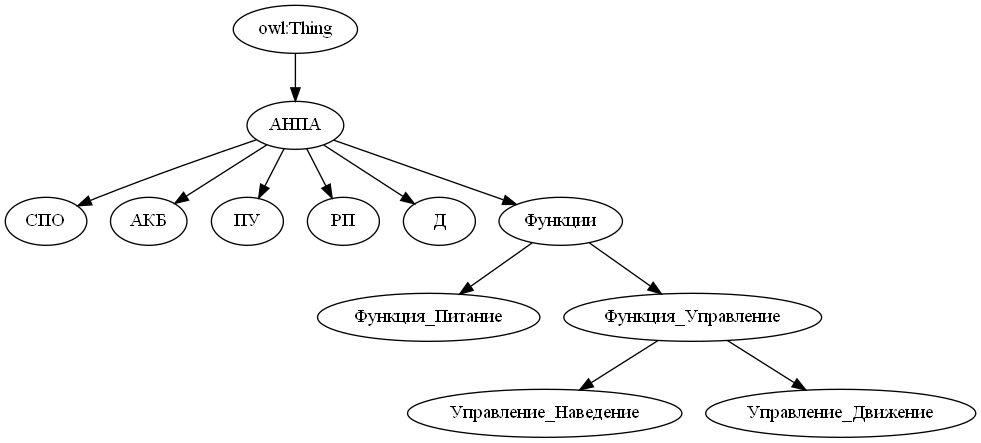
\includegraphics[width=.88\textwidth,keepaspectratio]{owl/anpa_hierarchy.png}
            %
            % 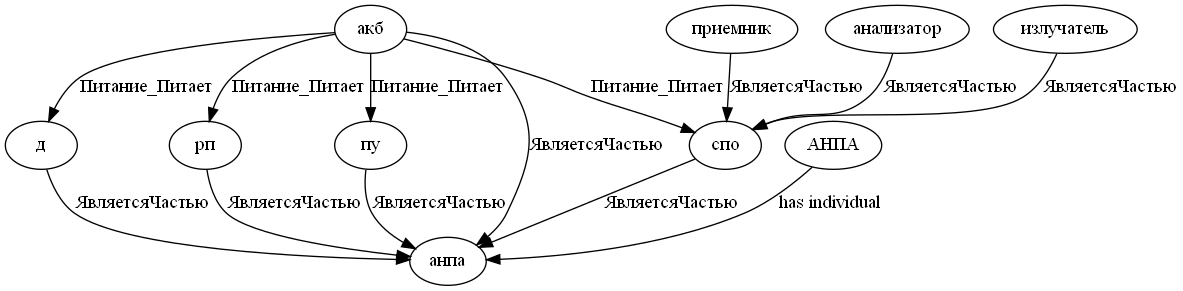
\includegraphics[width=.88\textwidth,keepaspectratio]{owl/part_of.png}
            %
            % \includegraphics<2->[width=.88\textwidth,keepaspectratio]{owl/function_movement.png}
        \end{center}
\end{frame}
\note{
На графе показана взаимосвязь сущностей для реализации движения и наведения.
Очевидно, что изменение, например, текущей глубины $h$ через \texttt{заглубиться} -- экземпляр класса \texttt{Управление\_Наведение},
происходит с участием ПУ через триплет <<заглубиться -- Функционал\_Наведение -- пу>>.
А это в свою очередь связано с работой СПО через экземпляры \textit{излучатель}, \textit{приемник} и \textit{анализатор}.
}



\section[Результат]{Программная реализация}



% \begin{frame}
%     \frametitle{Разделяющие линии}
%     \begin{minipage}[c]{0.47\linewidth}
%         \center{\includegraphics[width=1\linewidth]{logo}}
%         \bigskip
%         \hrule{}
%         \bigskip
%         \textbf{Составная \\ подпись 1}
%     \end{minipage}
%     \hfill
%     \vrule{}
%     \hfill
%     \begin{minipage}[c]{0.47\linewidth}
%         \flushright
%         \textbf{Составная \\ подпись 2}
%         \center{\includegraphics[width=1\linewidth]{logo}}
%     \end{minipage}
% \end{frame}

% \begin{frame}[allowframebreaks]
%     \frametitle{Уравнения Максвелла}
%     \centering{
%         \small
%         \def\arraystretch{1.8}%
%         \begin{tabular}{ll}
%             \toprule
%             Интегральная форма                                                                                                                                          & Дифференциальная форма                                                        \\ \midrule
%             \(Q_e(t) = \displaystyle\oiint_S \vec D(t) \cdot d\vec{s} = \displaystyle\iiint_V \rho_v(t) dv\)                                                              & \(\nabla \cdot \vec D(t) = \rho_v(t)\)                                          \\
%             \(\displaystyle\oiint_S \vec B(t) \cdot d\vec{s} = 0\)                                                                                                        & \(\nabla \cdot \vec B(t) = 0\)                                                  \\
%             \(V_{emf}(t) = \displaystyle\oint_L \vec E(t) \cdot d\vec{l}\) = \(- \displaystyle\iint_S \left[\frac{\partial\vec{B}(t)}{\partial t}\right] \cdot d\vec{s}\)   & \(\nabla \times \vec E(t) = - \frac{\partial\vec{B}(t)}{\partial t}\)           \\
%             \(I(t) = \displaystyle\oint_L \vec H(t) \cdot d\vec{l} = \displaystyle\iint_S \left[\vec J(t) + \frac{\partial\vec{D}(t)}{\partial t}\right] \cdot d\vec{s}\) & \(\nabla \times \vec H(t) = \vec J(t) + \frac{\partial\vec{D}(t)}{\partial t}\) \\ \midrule
%             \(\displaystyle\oiint_S \vec J \cdot d\vec{s} = -\frac{\partial Q_e}{\partial t}\)                                                                            & \(\nabla \cdot \vec J = - \frac{\partial \rho_v}{\partial t}\)                  \\
%             \bottomrule
%             \multicolumn{2}{c}{\(\vec D(t) = \left[\varepsilon(t)\right] * \vec E(t)\)}                                                                                                                                                                   \\
%             \multicolumn{2}{c}{\(\vec B(t) = \left[\mu(t)\right] * \vec H(t)\)}                                                                                                                                                                           \\
%         \end{tabular}
%     }
%     \framebreak

%     \hspace{0.05\linewidth}
%     \centering{
%         \small
%         \def\arraystretch{1.8}%
%         \begin{tabular}{ll}
%             \toprule
%             Интегральная форма                                                                                                            & Дифференциальная форма                             \\ \midrule
%             \(Q_e = \displaystyle\oiint_S \vec D \cdot d\vec{s} = \displaystyle\iiint_V \rho_v dv\)                                         & \(\nabla \cdot \vec D = \rho_v\)                     \\
%             \(\displaystyle\oiint_S \vec B \cdot d\vec{s} = 0\)                                                                             & \(\nabla \cdot \vec B = 0\)                          \\
%             \(V_{emf} = \displaystyle\oint_L \vec E \cdot d\vec{l}\) = \(- \displaystyle\iint_S \left[j \omega \vec B\right] \cdot d\vec{s}\) & \(\nabla \times \vec E = - j \omega \vec B\)         \\
%             \(I = \displaystyle\oint_L \vec H \cdot d\vec{l} = \displaystyle\iint_S \left[\vec J + j \omega \vec D\right] \cdot d\vec{s}\)  & \(\nabla \times \vec H = \vec J + j \omega \vec{D}\) \\ \midrule
%             \(\displaystyle\oiint_S \vec J \cdot d\vec{s} = - j \omega Q_e\)                                                                & \(\nabla \cdot \vec J = - j \omega \rho_v\)          \\
%             \bottomrule
%             \multicolumn{2}{c}{\(\vec D(t) = \left[\varepsilon\right] \vec E(t)\)}                                                                                                               \\
%             \multicolumn{2}{c}{\(\vec B(t) = \left[\mu\right] \vec H(t)\)}                                                                                                                       \\
%         \end{tabular}
%     }
% \end{frame}

% \begin{frame}
%     \frametitle{Другая таблица}
%     \centering
%     \begin{tabular}{lc}
%         \toprule
%         \multicolumn{1}{c}{\textbf{Заголовок 1}} & \textbf{Заголовок 2} \\ \midrule
%         Сумма                                    & \(b+a\)                \\
%         Разность                                 & \(a-b\)                \\
%         Произведение                             & \(a*b\)                \\
%         \bottomrule
%     \end{tabular}
% \end{frame}
